% !TeX spellcheck = ru_RU
\chapter{Выполнение лабораторной работы}

\section{Цель работы}

Лабораторная работа № 5 нацелена на освоение возможностей программы Microsoft Project по управлению финансовыми потоками на основе анализа затрат.

\section{Краткое описание проекта}

Команда разработчиков из 16 человек занимается созданием карты города на основе собственного модуля отображения. Проект должен быть завершен в течение 6 месяцев. Бюджет проекта: 50 000 рублей.

\section{Задание 1}

Таблица освоенного объема состояния проекта после выполнения шага 7 лабораторной работы 4 представлена на рисунке~\ref{fig:1}. Дата отчета~---~10 мая.

\begin{figure}[H]
	\centering
	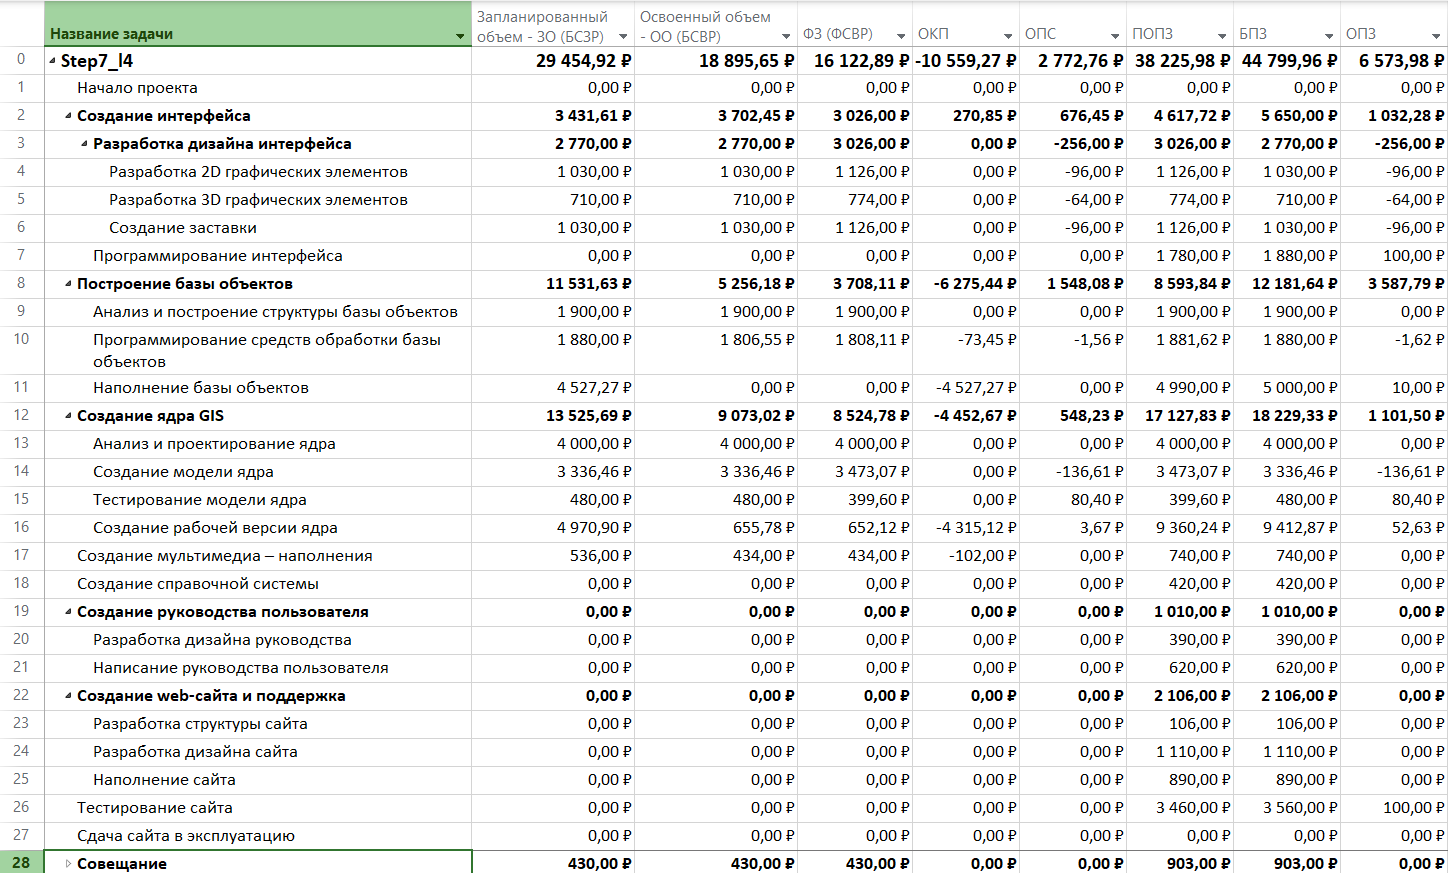
\includegraphics[width=\linewidth]{images/start.png}
	\caption{Таблица освоенного объема проекта}
	\label{fig:1}
\end{figure}

Причины отклонения ОКП и ОПС по задачам:
\begin{itemize}
	\item в задаче №3 "Разработка дизайна интерфейса" ненулевой ОПС (-256 рублей) связан с 10\% увеличение трудозатрат по ее подзадачам;
	\item в задаче №10 "Программирование средств обработки базы объектов" ненулевой ОКП (-73,45 рублей) связан с отставанием задачи от плана: плановое завершение 20.04, на 10.05 задача завершена на 96\%;
	\item в задаче №10 "Программирование средств обработки базы объектов" ненулевой ОПС (-1,56 рублей) связан с увеличением оплаты программистам 2 и 4 на время командировки программистов 1 и 3;
	\item в задаче №11 "Наполнение базы объектов" ненулевой ОКП (-4 527,27 рублей) связан с отставанием задачи от плана: плановое завершение 13.05, на 10.05 задача завершена на 0\%;
	\item в задаче №14 "Создание модели ядра" ненулевой ОПС (-136,61 рублей) также связан с увеличением оплаты программистам 2и 4 на время командировки программистов 1 и 3;
	\item в задаче №15 "Тестирование модели ядра" ненулевой ОПС (80,4 рублей) также связан с увеличением оплаты программистам 2и 4 на время командировки программистов 1 и 3;
	\item в задаче №16 "Создание рабочей версии ядра" ненулевой ОКП (-4 315,12) обоснован отставанием задачи от сроков: плановое начало 08.04, фактическое~---~28.04;
	\item в задаче №17 "Создание мультимедиа-наполнения" ненулевой ОКП (-102) также связан с отставанием задачи от плана: плановое начало 07.04, фактическое~---~13.04.
\end{itemize}

Несмотря на перечисленные отрицательные показатели ОПС, по всему проекту на 10.05 ОПС положителен и составляет 2772,76 рублей, что свидетельствует об экономии финансовых средств относительно плана. Тем не менее отрицательный ОКП по проекту -10 599,27 рублей при запланированном объеме в 29 454,92 свидетельствует о том, что проект отстает (и очень сильно) от плана. Показатель ОПЗ составляет 6 573,98 рублей, таким образом по завершении предварительно перерасход средств не предполагается.

\section{Задание 2}

Для определения недели на которой будет наибольшая потребность в деньгах был построен отчет, диаграмма представлена на рисунке~\ref{fig:2}. Исходя из нее, наибольшая необходимость в денежных средствах будет приходиться на 5-ую неделю.

\begin{figure}[H]
	\centering
	
\includegraphics[width=\linewidth]{images/babki.png}
	\caption{Диаграмма отчета о движении денежных средств}
	\label{fig:2}
\end{figure}

Диаграмма отклонения стоимостей задач представлена на рисунке~\ref{fig:3}. Задачи создания интерфейса и построения базы объектов значительно превышают бюджет (на 1400 и 3900 рублей соответственно). Задача тестирования сайта имеет запас в 100 рублей.

\begin{figure}[H]
	\centering
	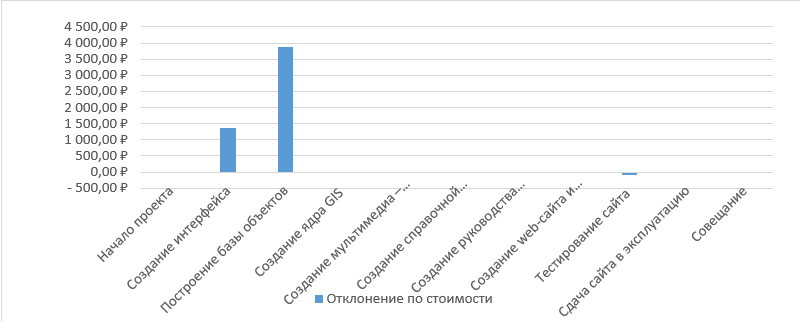
\includegraphics[width=\linewidth]{images/wasted.png}
	\caption{Диаграмма отклонений стоимостей задач}
	\label{fig:3}
\end{figure}

\section{Задание 3}

Измененная декомпозиция работ проекта, основанная на каскадной модели жизненного цикла приведена на рисунке~\ref{fig:4}, исходная на рисунке~\ref{fig:5}. Измененная декомпозиция после автоматического разрешения перегрузок представлена на рисунке~\ref{fig:6}.

\begin{figure}[H]
	\centering
	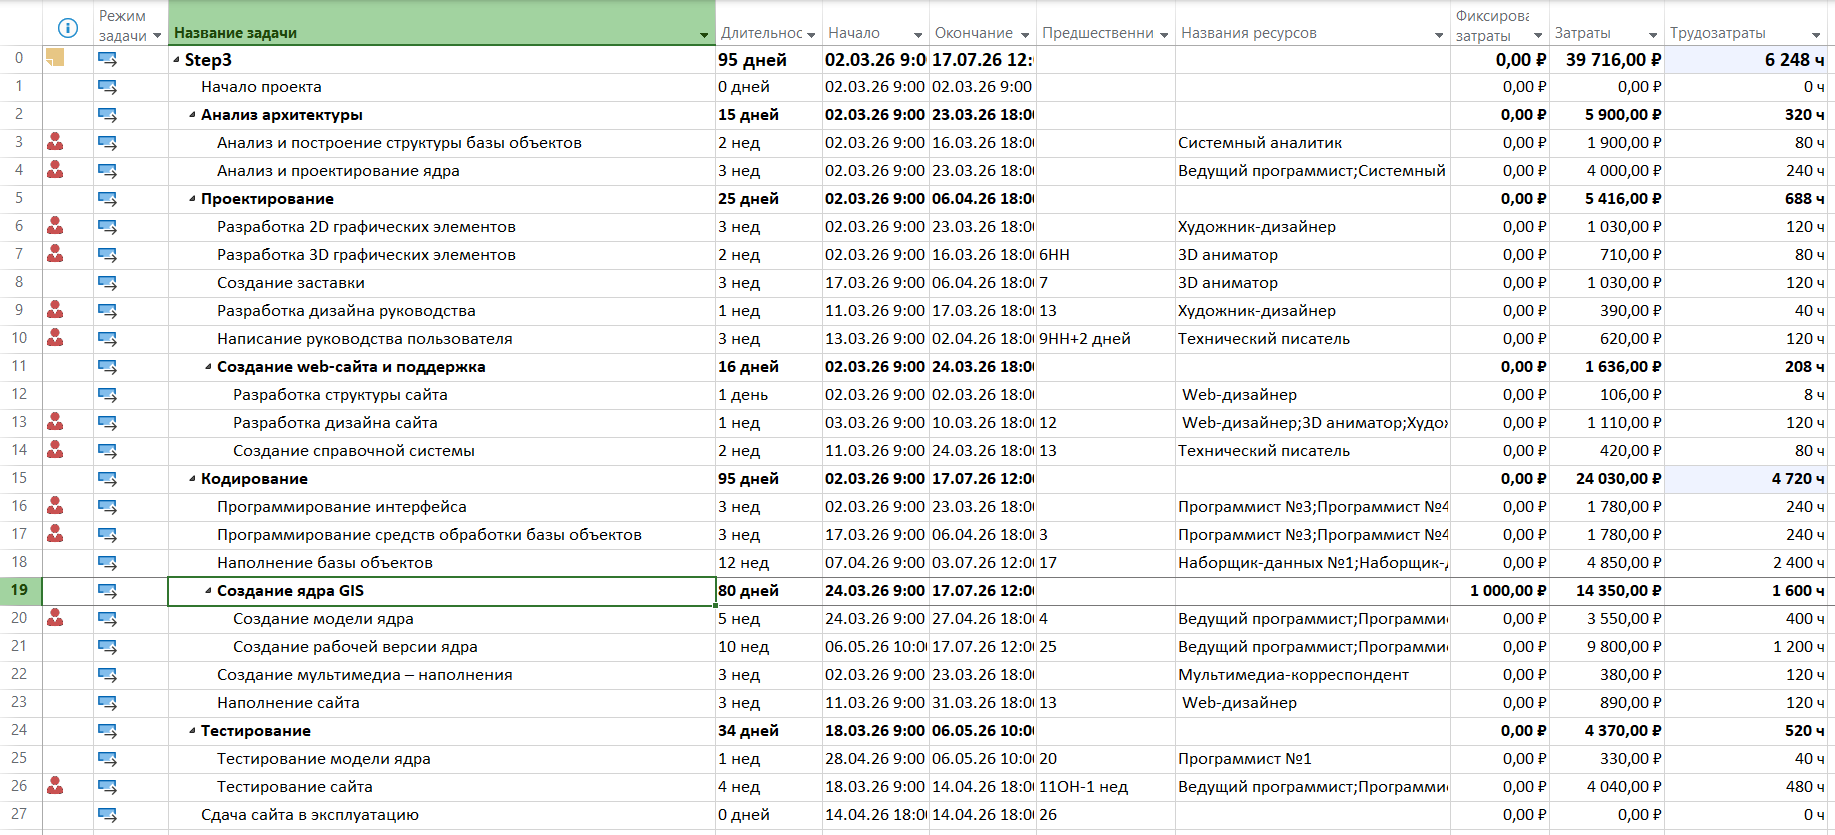
\includegraphics[width=\linewidth]{images/recompose_over.png}
	\caption{Измененная декомпозиция задач проекта}
	\label{fig:4}
\end{figure}

\begin{figure}[H]
	\centering
	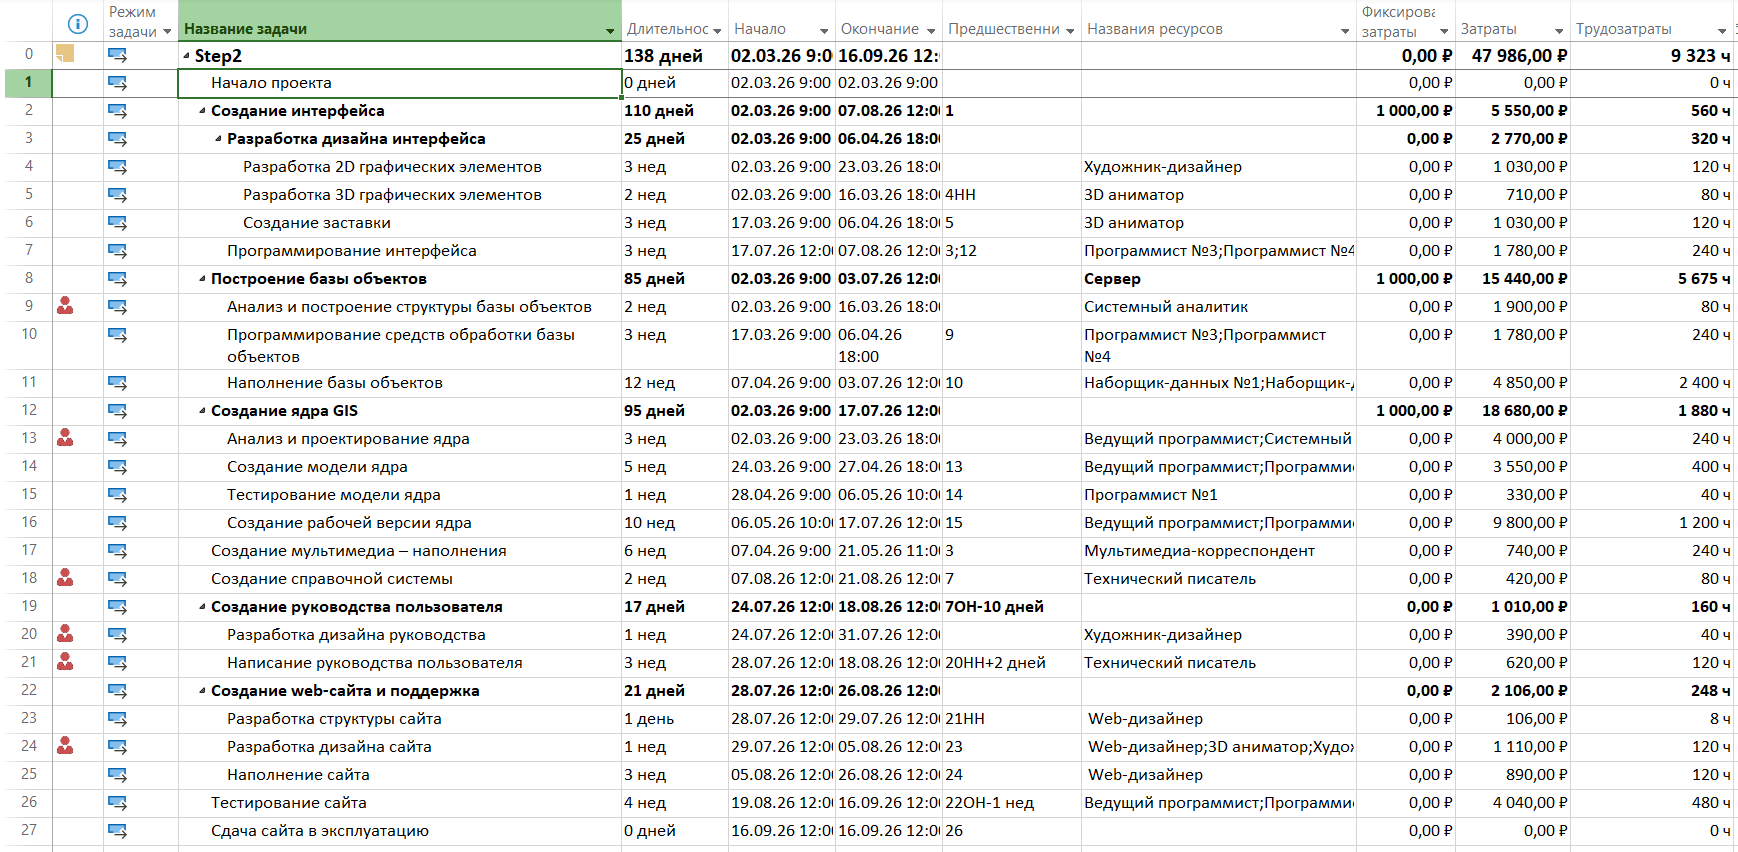
\includegraphics[width=\linewidth]{images/source.png}
	\caption{Исходная декомпозиция задач проекта}
	\label{fig:5}
\end{figure}

\begin{figure}[H]
	\centering
	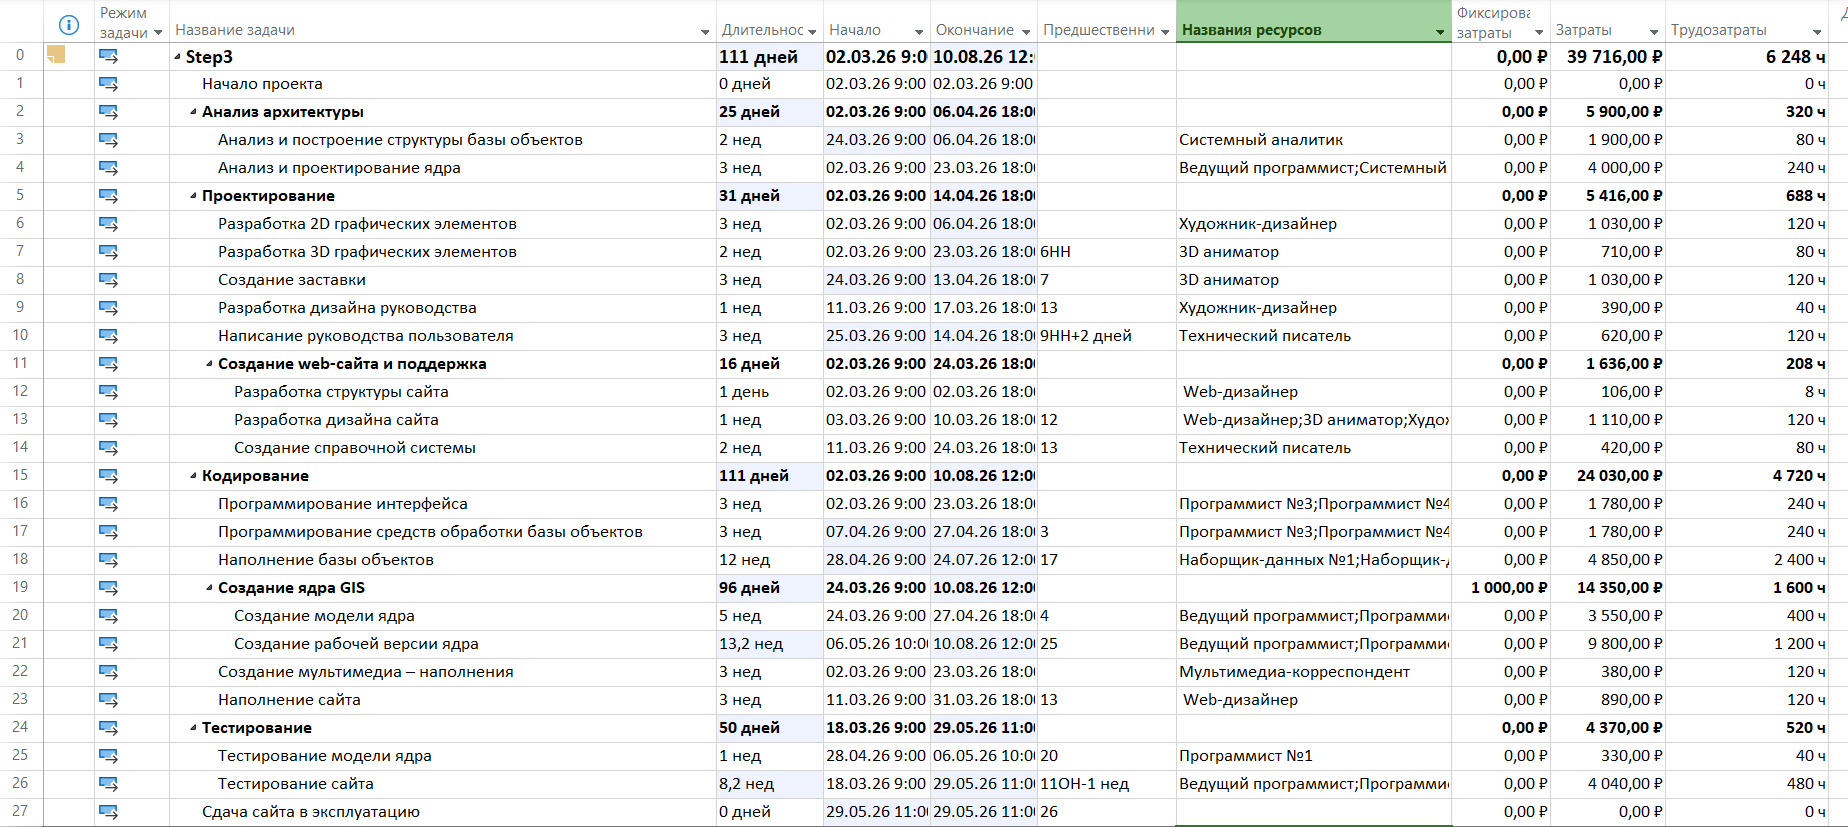
\includegraphics[width=\linewidth]{images/no_over.png}
	\caption{Измененная декомпозиция задач проекта после разрешения перегрузок}
	\label{fig:6}
\end{figure}

Исходя из полученных данных, каскадная модель позволяет сэкономить более месяца работ (дата окончания 10.08 вместо 16.09), и 8 270 рублей (39 716 вместо 47 986 рублей). Основным недостатком каскадной модели является необходимость заранее тщательно спроектировать систему, в связи с высокой сложностью дальнейшего изменения требований.